\documentclass[12pt]{exam}
\usepackage[utf8]{inputenc}
\usepackage[francais]{babel}
\usepackage{a4wide}
\usepackage{graphicx}
\usepackage{algorithm}
\usepackage{algorithmic}
\usepackage{color}
\usepackage{fourier-orns}
\usepackage{listings}
\lstset{language=java}


\printanswers


\title{TP de prise en main de la bibliothèque MG2D}
\author{Rémi Synave}
\date{}


\begin{document}
\maketitle
\tableofcontents

\newpage

\section{MG2D}
MG2D (Moteur Graphique 2D) est une bibliothèque java permettant de créer facilement des fenêtres graphiques dans lesquelles peuvent être affichées des primitives géométriques simples, du texte ou des textures. Elle permet également de gérer les collisions entre les primitives. Finalement, tous les commentaires et la documentation sont en Français.

La bibliothèque va vous permettre de créer des programmes graphiques simples ou des petits jeux au look rétro. N'espérez pas coder le prochain fifa ! L'affichage n'est pas optimisé et la création de programme dynamique demandera l'utilisation d'artifices basiques. Ceci sera expliqué dans ce document.

Dans ce document, vous pourrez également trouver :
\begin{itemize}
\item les instructions pour installer la bibliothèque (si vous ne l'avez pas encore fait),
\item une description rapide des classes \texttt{Fenetre}, \texttt{Clavier} et \texttt{Souris}. Vous trouverez toutes les informations complémentaires dans la documentation (voir les instructions d'installation de la bibliothèque pour la génération de la documentation),
\item plusieurs exemples de programme,
\item un ensemble d'exercices pour prendre en main la bibliothèque.
\end{itemize}

\section{Pré-requis}
\subsection{Installation de la bibliothèque sous linux}
\label{install}
Si vous avez déjà suivi les instructions d'installation, vous pouvez passer cette partie et aller directement en section~\ref{import}.

Dans le cas contraire, voici les instructions à suivre :
\begin{enumerate}
\item Ouvrez un terminal et éditer votre fichier \texttt{.bashrc} (si vous êtes sous linux. Sinon sous mac, ce sera le fichier ~/.bash\_profile) :\\
\texttt{emacs $\sim$/.bashrc}

Ajoutez la ligne suivante tout en bas du fichier :\\
\texttt{export CLASSPATH=\$CLASSPATH:$\sim$/}

Fermez votre terminal et relance le.

\item Dans votre terminal, déplacez vous dans le répertoire 
créé lorsque que vous avez décompressé l'archive. Déplacez le répertoire MG2D à la racine de votre dossier personnel :\\
\texttt{mv MG2D $\sim$}

Déplacez vous dans ce répertoire et compilez la bibliothèque et la doc :\\
\texttt{cd $\sim$/MG2D}\\
\texttt{make}\\
La documentation se trouve dans le répertoire \texttt{doc} qui vient d'être créé.

\item Vous pouvez tester les trois jeux disponibles dans le répertoire décompressé \texttt{Demos/Kowasu\_Renga}, \texttt{Demos/Snake\_Eater} et \texttt{Demos/Pong} ainsi que les différents fichiers de test dans le répertoire \texttt{Demos/Test\_MG2D}.
\end{enumerate}

\subsection{Importation dans les programmes}
\label{import}
Pour pouvoir utiliser les classes et fonctionnalités de la bibliothèque MG2D, après installation (voir section~\ref{install}, vous devrez importer la bibliothèque comme ceci :
\begin{lstlisting}
import MG2D.*;
import MG2D.geometrie.*;
\end{lstlisting}
Ces deux lignes sont à placer en tout début de fichier (avant même la déclaration de la classe), dans chaque classe utilisant la bibliothèque.

\section{La classe \texttt{Fenetre}}
Dans un programme, le fait d'instancier un objet de type \texttt{Fenetre} crée une fenêtre graphique vide (avec un fond blanc). Le constructeur est le suivant :\\
\texttt{Fenetre(String titre, int largeur, int hauteur)}\\
Le premier paramètre est le titre de votre fenêtre. Les deux paramètres suivants sont la taille de votre fenêtre en largeur et en hauteur.\\

L'origine de la fenêtre créée se trouve en bas à gauche (comme dans les repères en mathématiques).\\

La méthode \texttt{rafraichir} permet de mettre à jour l'affichage. La fenêtre créée est vide. Pour afficher des primitives, il faut les instancier, les ajouter à la fenêtre et mettre à jour l'affichage. Si les objets ont changé de place ou de couleur depuis la dernière mise à jour de l'affichage, l'appel à cette méthode permet la réactualisation du contenu de la fenêtre.\\

Un objet de type \texttt{Fenetre} permet également les opérations suivantes (voir doc pour plus de détails) :
\begin{itemize}
\item ajouter des primitives,
\item supprimer des primitives,
\item effacer la fenêtre,
\item trouver facilement le centre de la fenêtre,
\item faire des captures d'écran.
\end{itemize}

\section{Programme minimal statique}
Ce programme vous permettra de savoir si la bibliothèque est bien installée et le système correctement configuré.

\begin{lstlisting}
import MG2D.*;

class Main{
  public static void main(String[] args){
    Fenetre f = new Fenetre("Mon appli MG2D", 800, 600);
  }
}
\end{lstlisting}

Ce programme doit afficher une fenêtre vide comme en figure~\ref{fig}.

\begin{figure}[htbp]
  \centering
  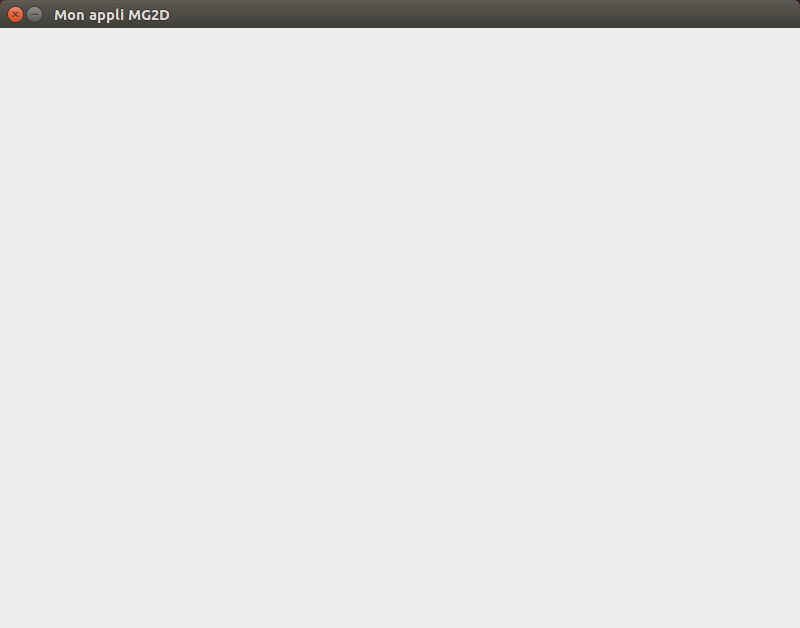
\includegraphics[width=10cm]{./images/appliMG2Dstatique}
  \caption{\label{fig}Fenête vide.}
\end{figure}

\section{La classe \texttt{Clavier}}
La bibliothèque offre la possibilité de contrôler les applications créées grâce au clavier. Vous pourrez gérer des événements clavier très simple. Les événements gérés sont l'appui sur l'une des touches suivantes : a/z/e/q/s/d/espace/entrée et les flèches directionnelles.
L'appel à la méthode \texttt{getClavier} sur un objet de type \texttt{Fenetre} donne accès à la gestion des touches pour cette fenêtre. Un objet de type \texttt{Clavier} est retourné. C'est cet objet qui nous permet de tester l'appui sur l'une des touches citées précédemment (voir documentation pour le détail des méthodes).

Si la gestion du clavier ne convient pas à votre application, il vous est toujours possible de créer votre propre classe \texttt{Clavier} (en prenant modèle sur la classe existante si vous le voulez). Afin d'avoir accès au clavier grâce à votre classe, vous devrez produire le code suivant (à adapter en fonction de vos noms d'instance).
\begin{lstlisting}
Fenetre f = new Fenetre("mon appli", TAILLEX, TAILLEY);
Clavier clavier = new Clavier();
f.addKeyListener(clavier);
\end{lstlisting}

\section{La classe \texttt{Souris}}
La bibliothèque offre la possibilité de contrôler les applications créées grâce à la souris. Vous pourrez gérer des événements souris très simple. Il est possible de tester si les clics gauche/droit/milieu sont enfoncés, s'il y a eu un clic gauche/droit/milieu ou de connaître la position du curseur.
.
L'appel à la méthode \texttt{getSouris} sur un objet de type \texttt{Fenetre} donne accès à la gestion de la souris pour cette fenêtre. Un objet de type \texttt{Souris} est retourné. C'est cet objet qui nous permet de tester les clics et la position du curseur (voir documentation pour le détail des méthodes).

Si la gestion de la souris ne convient pas à votre application, il vous est toujours possible de créer votre propre classe \texttt{Souris} (en prenant modèle sur la classe existante si vous le voulez). Afin d'avoir accès à la souris grâce à votre classe, vous devrez produire le code suivant (à adapter en fonction de vos noms d'instance).
\begin{lstlisting}
Fenetre f = new Fenetre("mon appli", TAILLEX, TAILLEY);
Souris souris = new Souris(TAILLEY);
f.addMouseListener(souris);
f.addMouseMotionListener(souris);
\end{lstlisting}
\danger \textbf{Si vous développez votre propre classe \texttt{Souris}, l'origine de la fenêtre se trouvera en haut à gauche. C'est donc à vous de gérer ceci dans votre application ou, mieux, dans votre classe \texttt{Souris}.}

\section{\texttt{Clavier} et \texttt{Souris} par défaut}
Si le comportement du clavier et de la souris par défaut vous conviennent, vous pouvez remplacer le code des deux sections précédentes par :
\begin{lstlisting}
Fenetre f = new Fenetre("mon appli", TAILLEX, TAILLEY);
Clavier clavier = f.getClavier();
Souris souris = f.getSouris();
\end{lstlisting}

\section{Créer de la dynamique}
Dans une application, pour créer de la dynamique, il y a 2 possibilités :
\begin{itemize}
\item dynamisme continu comme dans \textit{tetris} où les pièces descendent en continu
\item dynamisme non continu (en réaction à des événements clavier ou souris par exemple) comme dans \textit{puissance4} où l'affichage n'est modifié que lorsqu'un joueur a placé un nouveau pion dans la grille.
\end{itemize}

\subsection{Dynamisme continu}
Dans ce cas, pour créer de la dynamique, il vous faudra une boucle dans laquelle seront mis à jour tous les éléments affichés. Comme il a été dit précédemment, aucune optimisation ni régulation de l'affichage (au niveau du nombre d'images par seconde - FPS) n'est implémentée. Or, ces modifications de position et/ou de couleur des primitives se feront très rapidement. Ceci entrainera forcément un nombre de FPS très élevé et une vitesse d'exécution trop rapide. Afin de limiter les FPS et obtenir une vitesse d'exécution correcte, il vous faudra gérer des petites pauses dans vos programmes : les quelques lignes suivantes vous permettent de faire des pauses de $20ms$.
  
\begin{lstlisting}
try{
  Thread.sleep(20);
}
catch(Exception e){
}
\end{lstlisting}
En fonction de l'effet souhaité, du nombre de primitives affichés il vous faudra adapter le temps de pause. Vous pouvez également tenter d'estimer, dans votre programme, le temps mis par la boucle pour faire un tour et ainsi calculer le bon temps de pause. Ceci vous permettra d'avoir une animation fluide et sans ralentissement et/ou accélération.

Vous pourrez trouver un exemple de programme dynamique continu en annexe (voir section~\ref{dynContinu}).

\subsection{Dynamisme non continu}
Dans ce cas, vous allez devoir attendre un événement. Ceci implique la création d'une boucle qui ne fait rien et dont la condition de fin sera la survenue de l'événement. Afin de ne pas faire tourner votre processeur dans le vide, vous allez devoir utiliser le même morceau de code que précédemment que nous allons adapter à une boucle d'attente :
\begin{lstlisting}
while(!souris.getClicGauche()){
  try{
    Thread.sleep(1);
  }
  catch(Exception e){}
}
\end{lstlisting}

Vous pourrez trouver un exemple de programme dynamique non continu en annexe (voir section~\ref{dynNonContinu}).

\newpage

\section{Exercices pour la prise en main de la bibliothèque}
\subsection{Exercice1}
Créez un programme permettant de reproduire la figure~\ref{ex1}.

\begin{figure}[htbp]
  \centering
  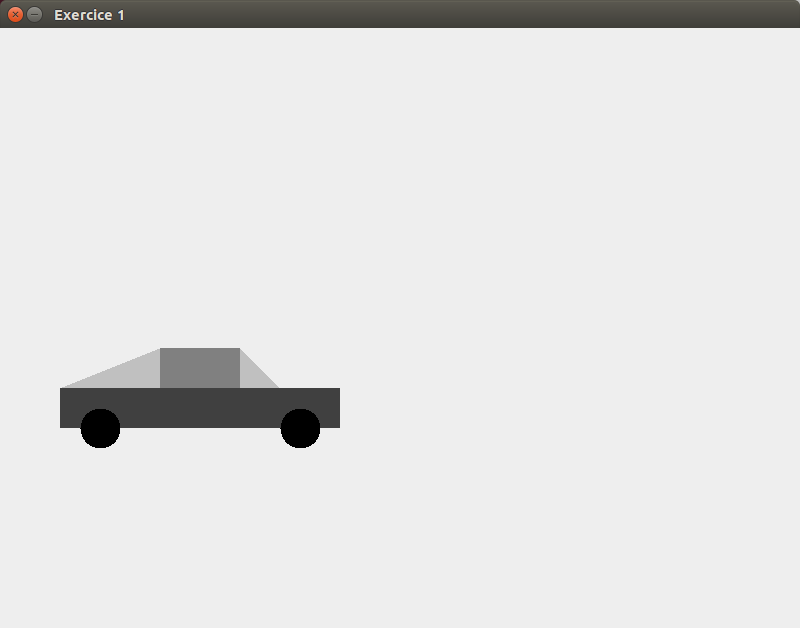
\includegraphics[width=10cm]{./images/Exercice1}
  \caption{\label{ex1}Ma jolie DeLorean.}
\end{figure}

\subsection{Exercice2}
A votre programme précédent, ajoutez du mouvement sur la voiture. Faites la rouler vers la droite. Lorsqu'elle sort de la fenêtre, faîtes la réapparaitre sur la gauche de la fenêtre.

Pour vous faciliter le travail : chaque primitive géométrique possède une méthode \texttt{translater} (voir la documentation).

\subsection{Exercice3}
A votre programme précédent, ajoutez la possibilité de modifier la vitesse de la voiture. La vitesse augmentera (respectivement diminuera) lorsque la flèche du haut (respectivement flèche du bas) sera pressée.

\subsection{Exercice4}
A votre programme précédent, ajoutez le changement de couleur de la carosserie lors d'un clic gauche. La couleur passera du gris au rouge.


\newpage
\section{ANNEXES}
\subsection{Exemple de programme dynamique continu}
\label{dynContinu}
\begin{lstlisting}
//Importation de la bibliotheque
import MG2D.*;
import MG2D.geometrie.*;

class DynamismeContinu{

  public static void main(String[] args){
    //Creation de la fenetre et de la gestion du clavier
    Fenetre f = new Fenetre ("Mon appli MG2D", 800, 600);
    Clavier clavier = f.getClavier();

    //Ajout d'un cercle bleu dans la fenetre
    Cercle c = new Cercle (Couleur.BLEU, new Point (200,100),5,true);
    f.ajouter(c);
	
    //Boucle infinie tournant sans arret
    while(true){
      //pause de 40ms
      try{
        Thread.sleep(40);
      }
      catch(Exception e){}
	 
      int x = c.getO().getX()-200;
      int y = c.getO().getY()-100;
      //On fait avancer le cercle de 2 vers la droite
      x=(x+2)%400;
	    
      //Si la fleche du haut est presse, on fait monter le cercle
      if(clavier.getHaut())
        y=(y+50)%500;
      
      c.setO(new Point(x+200,y+100));
      f.rafraichir();
    }
  }
  
}
\end{lstlisting}
\newpage
\subsection{Exemple de programme dynamique non continu}
\label{dynNonContinu}
\begin{lstlisting}
//Importation de la bibliotheque
import MG2D.*;
import MG2D.geometrie.*;

class DynamismeNonContinu{

  public static void main(String[] args){
    //Creation de la fenetre et de la gestion de la souris
    Fenetre f = new Fenetre ("Mon appli MG2D", 800, 600);
    Souris souris = f.getSouris();

    int indice=0;
    
    //On va creer 10 points dans la fenetre
    while(indice<10){
      //On attend un clic gauche
      while(!souris.getClicGauche()){
        try{
          Thread.sleep(1);
        }
        catch(Exception e){}
      }
      
      //On recupere la position de la souris
      Point p=new Point(souris.getPosition());
      
      //On cree un cercle bleu a l'endroit du clic de rayon 5
      Cercle c=new Cercle(Couleur.BLEU, p, 5, true);  
      //On ajoute ce cercle a la fenetre
      f.ajouter(c); 
      //On met a jour l'affichage
      f.rafraichir();
      
      indice++;
    }
  }
    
}
\end{lstlisting}
\end{document}
